The message signal is available in 
\begin{lstlisting}
/fm/msg/codes/Sound_Noise.wav
\end{lstlisting}
\begin{enumerate}[label=\arabic*.,ref=\thesection.\theenumi]
\numberwithin{equation}{enumi}
\item Plot the spectrum of the message signal using the builtin FFT algorithm.\\
	\solution		
\begin{figure}[H]
\centering
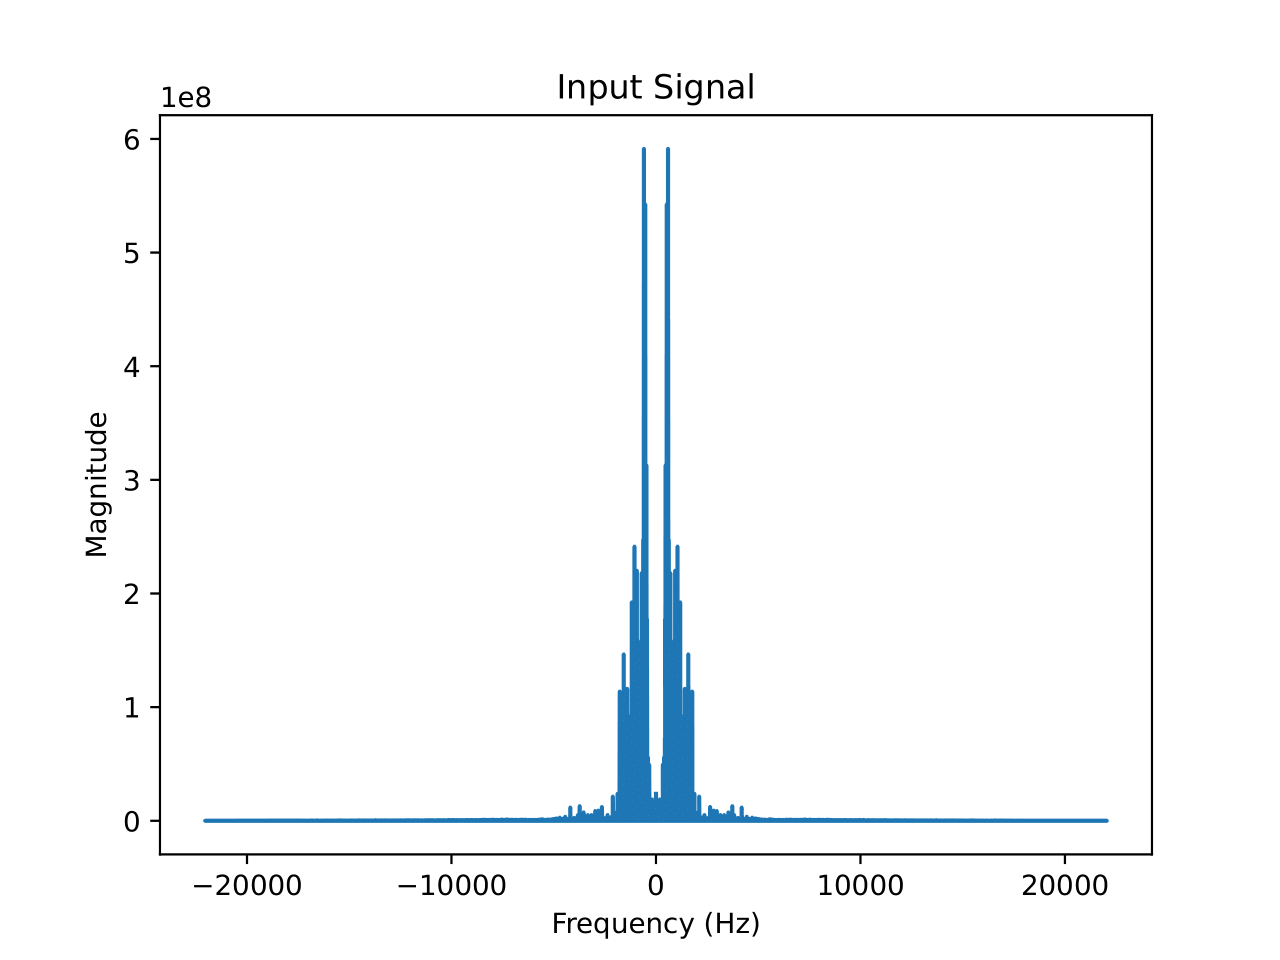
\includegraphics[width=\columnwidth]{fm/msg/figs/FFTbuiltin/inputs-1.png}
\caption{Plot of spectrum of message signal using builtin FFT algorithm.}
\label{fig:FFTb}
\end{figure}
The folowing code plots the spectrum in \figref{fig:FFTb} using the builtin FFT algorithm of the python library 'Numpy.'
\begin{lstlisting}
/fm/codes/input.py
\end{lstlisting}
\\
\item Plot the spectrum of the message signal by writing your own FFT algorithm.
	\\
	\solution
		\begin{figure}[H]
		\centering
		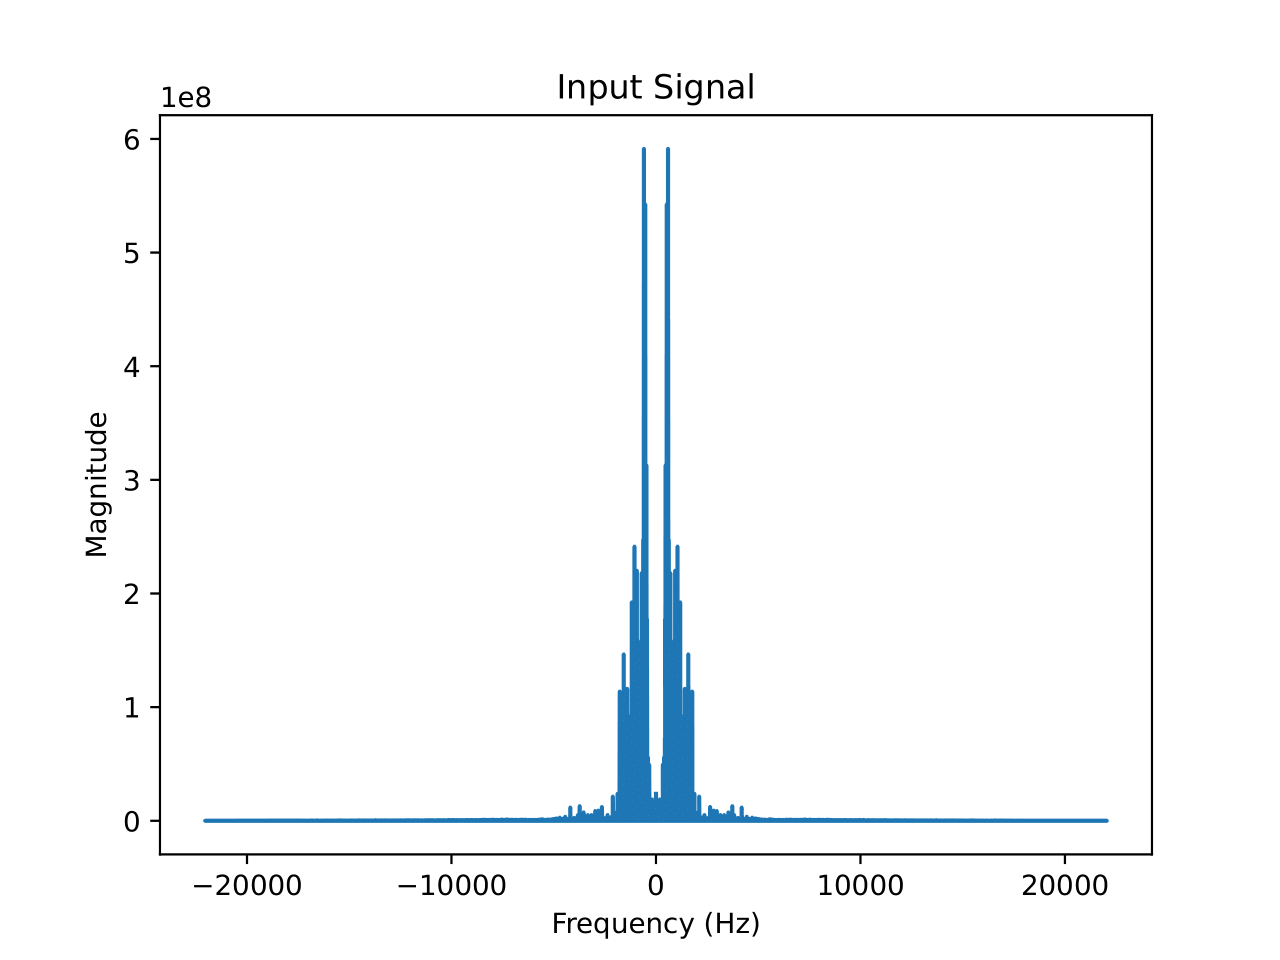
\includegraphics[width=\columnwidth]{fm/msg/figs/FFTown/input2.png}
		\caption{Plot of spectrum of message signal using own FFT algorithm.}
		\label{fig:FFTo}
		\end{figure}
		The folowing code plots the spectrum in \figref{fig:FFTo} using the DFT defined in  
	\eqref{eq:app-dft-def}.
\begin{lstlisting}
/fm/msg/codes/FFTmsg.py
\end{lstlisting}

\item Find the bandwidth of the message signal.\\
\solution The bandwidth can be calculated mathematically using the following formula:
\begin{align*}
B=mask_{maxi}-mask_{min}
\end{align*}
where $mask_{maxi}$ and $mask_{min} $ are the maximum amd minimum frequency bounds of the range  respectively.\\
Analyzes the audio signal and plots its magnitude spectrum. The bandwidth of the audio signal is  calculated using power spectral density. Obtain the bandwidth of the audio as 2 khz using below code
\begin{lstlisting}
/codes/input.py
\end{lstlisting}
\end{enumerate}
